

\section{The gem5 Simulator}

There is ``a new golden age for computer architecture''~\cite{turinglecture,cacm} driven by changes in technology (e.g., the slowdown of Moore's Law and Dennard Scaling) and ever increasing computational needs.
One of the first steps in research and development of new hardware architectures is software-based modeling and simulation.
The gem5 simulator~\cite{Binkert-gem5-2011} is currently one of the most popular academic-focused computer architecture simulation frameworks.
Since its publication in 2011, the gem5 paper has been cited over 3600 times\footnote{\url{https://scholar.google.com/scholar?q=gem5}}, and every year many papers published in the top computer architecture venues use gem5 as their main evaluation technique.

The gem5 simulator~\cite{Binkert-gem5-2011} is an open source community-supported computer architecture simulator system.
It consists of a simulator core and models for everything from out of order processors, to DRAM, to network devices.
The gem5 project consists of the gem5 simulator\footnote{\url{https://gem5.googlesource.com/public/gem5}}, documentation\footnote{\url{https://www.gem5.org/}}, and common resources\footnote{\url{https://gem5.googlesource.com/public/gem5-resources}} that enable computer architecture research.

The gem5 project is governed by a meritocratic, consensus-based community governance document\footnote{\url{https://www.gem5.org/governance/}} with a goal to provide a tool to further the state of the art in computer architecture.
%The goal of gem5 is to provide a tool to further the state of the art in computer architecture.
gem5 can be used for (but is not limited to) computer-architecture research, advanced development, system-level performance analysis and design-space exploration, hardware-software co-design, and low-level software performance analysis.
Another goal of gem5 is to be a common framework for computer architecture.
A common framework in the academic community makes it easier for other researchers to share workloads as well as models and to compare and contrast with other architectural techniques.

The gem5 community strives to balance the needs of its three categories of users: academic researchers, industry researchers, and students learning computer architecture.
For instance, gem5 strives to balance adding new features (important to researchers) and a stable code base (important for students).
Specific user needs important to the community are enumerated below:
\begin{itemize}
    \item Effectively and efficiently emulate the behavior of modern processors in a way that balances simulation performance and accuracy
    \item Serve as a malleable baseline infrastructure that can easily be adapted to emulate the desired behaviors
    \item Provide a core set of APIs and features that remain relatively stable
    \item Incorporate features that make it easy for companies and research groups to stay up to date with the tip and continue contributing to the project
    \item Additionally, the gem5 community is committed to openness, transparency, and inclusiveness.
\end{itemize}

In this paper, we discuss the current state of gem5.
We first discuss the past, present and future of gem5.
Then, we give an overview of gem5's main features available today and describe how to become a member of the gem5 community for researchers, students, and teachers.
Finally, we include a significant section which describes the major changes in gem5 in the past nine years since the initial gem5 release.
Each subsection was contributed by at least one of the people who developed that part of the simulator as noted in the footnotes.

It has taken a huge number of people to make gem5 what it is today.
One of the goals of this paper is to recognize the hard work on this community infrastructure which is often overlooked.
We have tried to include everyone who has contributed and documented all of the major changes.

\subsection{The past, present, and future of gem5}

The gem5 simulator was born when the m5 simulator~\cite{}(https://www.computer.org/csdl/magazine/mi/2006/04/m4052/13rRUxYIMRJ) created at University of Michigan merged with the GEMS simulator~\cite{}(Multifacet's General Execution-Driven Multiprocessor Simulator (GEMS) Toolset) from University of Wisconsin.
These were two academic-oriented simulators, neither of which had an open development community (both simulators had their source available for free\footnote{\url{https://sourceforge.net/projects/m5sim/}}\footnote{https://research.cs.wisc.edu/gems/home.html}, but did not have a community-oriented development process).
Both of these simulators were quite popular on their own.
The GEMS paper has been cited over 1800 times and the m5 paper has been cited over 1000 times.

Since its initial release nine years ago the gem5 simulator has been wildly successful.
In this time, the use of gem5 has exploded.
Although not a perfect metric, the gem5 paper has received over 3600 citations according to Google Scholar.

\begin{figure}
    \centering
    \begin{subfigure}{0.4\linewidth}
      \centering
      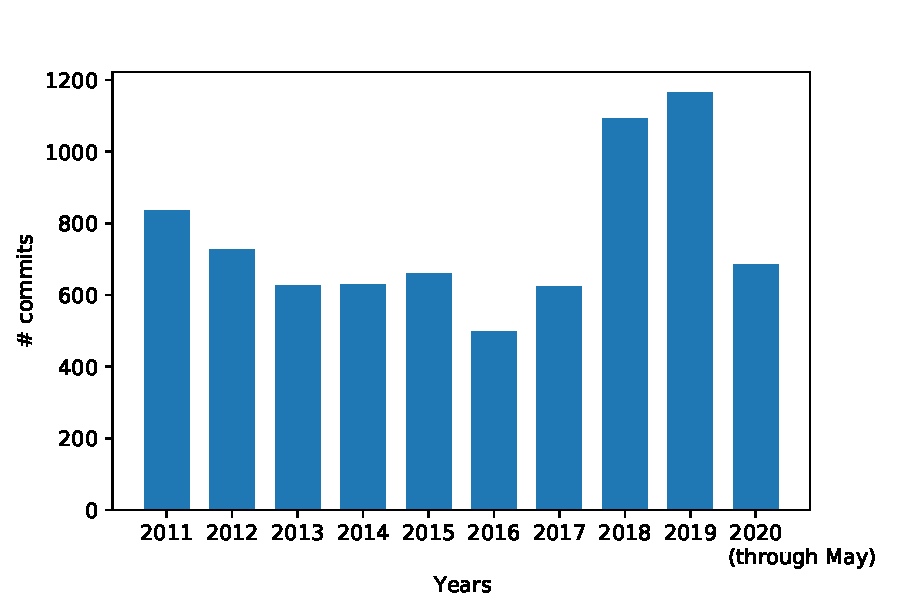
\includegraphics[height=4cm]{fig/gem5_commits}
      \caption{Number of commits}
      \label{fig:commits}
    \end{subfigure}
    \begin{subfigure}{0.4\linewidth}
      \centering
      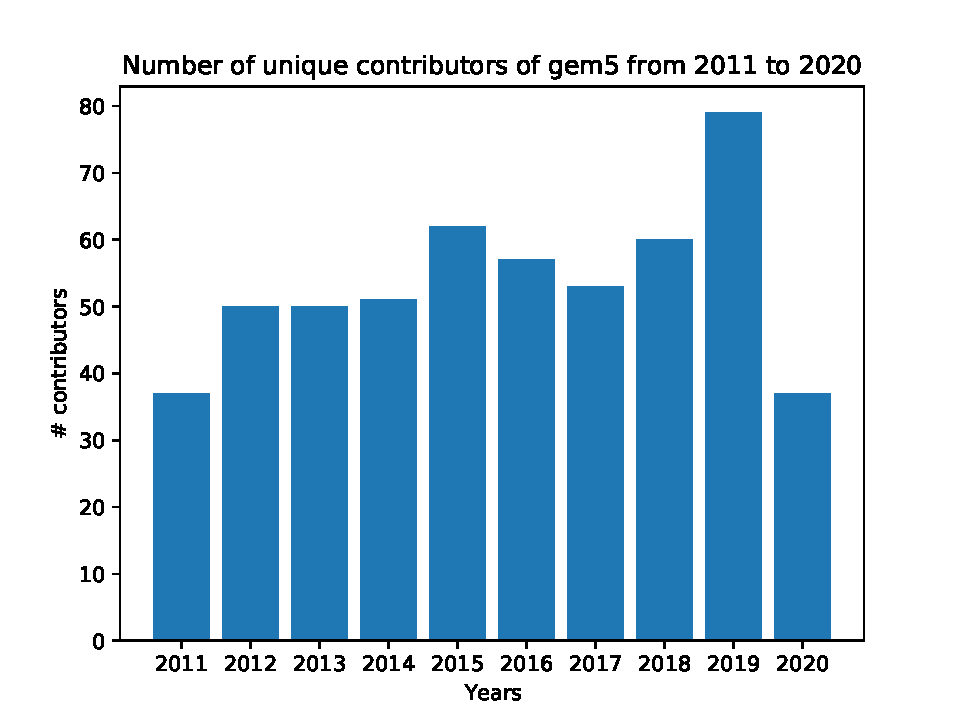
\includegraphics[height=4cm]{fig/gem5_contributors}
      \caption{Number of contributors}
      \label{fig:contributors}
    \end{subfigure}
    \caption{Number of gem5 commits and contributors from 2011 to 2020.}
    \label{fig:gem5_commits_contributors}
\end{figure}

At the same time, the contributor community has also grown.
Figures~\ref{fig:commits} shows the number of commits per year and Figure~\ref{fig:contributors} shows the number of unique contributors per year.
These figures show that since the initial release of gem5 in 2011, development has been significantly accelerating.

With this acceleration in use and development of gem5 came growing pains~\cite{Power-gem5horrors-2015}.
The gem5 community was going through a shift from a small project with most contributors from one or two academic labs to a project with worldwide-distributed contributors.
Additionally, given the growing user base, we could no longer assume that all gem5 users were also going to be main developers.

To solve these problems the gem5 community has made major changes in the past nine years.
We now have a formal governance structure, we have improved our documentation (see Section~\ref{sec:learning}), we have moved to a better distributed development platform, and improved our community outreach.

To institute a formal governance model, we followed the best practices from other successful open source projects.
We chose to institute a meritocratic governance model where anyone with an interest in the project can join the community, contribute to the project design and participate in the decision-making process.
The governance structure also defines the roles and responsibilities of members of the community including users, contributors, and maintainers.
We also formed a project management committee to help ensure smooth running of the project.
Importantly, members of the project management committee (PMC) do not have significant authority over other members of the community or of the direction of the project.

To simplify the contribution process, we have instituted many industry-standard development methodologies including providing a \verb|CONTRIBUTING| document in the gem5 source.
In the past, gem5 code contributions were managed with a number of esoteric software packages.
Now, all gem5 code is stored in a git repository\footnote{\url{googlesource}}, code review is managed on Gerrit\footnote{url{gem5-review}}, we have continuous integration support (see Section~\ref{sec:testing}), our website is implemented with jekyll and markdown\footnote{\url{gem5-website-repo}}, and we have a Jira-based issue tracker\footnote{\url{https://gem5.atlassian.net/}}.

After transitioning to these more well known tools and improved development practices, we have seen a rise in the number of community contributors and using gem5 has become frustrating.
Continuous integration enables us to test every single changeset before it is committed.
This allows us to catch bugs \emph{before} they are committed into the mainline repository which makes gem5 more stable.
Similarly, by implementing a bug tracking system, we can track issues that effect gem5.
In the first six months of using a bug tracker we have closed over 250 issues.

\subsubsection*{The future of gem5}
The future of gem5 is bright.
We will be continuing to work with the community to define the roadmap for gem5 development for gem5 version 20.1 and beyond.
In the short term, we are excited to to be improving the underlying infrastructure of gem5 with better testing, refactoring aging code (some of gem5's code is from 20 years ago!), and adding well-defined stable APIs.
By defining stable APIs, we will make it easier for the community to build off of gem5.
For instance, the inter-simulator interface is currently being defined so that gem5 can be used in conjuction with other simulators (e.g., SST~\cite{}, SystemC~\ref{sec:systemc}, and many others).
We are also working on improving the interconnect model~\ref{sec:garnet} and adding support for non-volatile memory controllers~\ref{sec:nvm}.

One of the most exciting features coming to gem5 is that we will provide the community with a set of \emph{publicly validated} models which will model current architectural system components including CPU cores, GPU compute units (CUs), caches, main memory systems, and devices.
We will strive for accuracy compared to real systems; however, since most systems are proprietary and complex, accuracy for all workloads will be difficult.
Thus, we will broadly advertise the relative performance, power, and other metrics when providing these models so users can make an informed decision when choosing their baseline configurations.
This will reduce the researcher's time spent on configuring baselines and allow them to concentrate more effort on analyzing and developing their novel research ideas.
The first step towards this goal of validated baselines is the gem5 resources repository described in Section~\ref{sec:resources}.

Finally, we are planning to publish an online ``Learning gem5'' course based on a largely expanded version of the Learning gem5 material~\ref{sec:learning}.
This course will cover how to get started using gem5, how to develop new models to be used in gem5, and the details of gem5's software architecture.
In addition to the online version of the course, we will continue to conduct tutorials and workshops at computer architecture and computer systems conferences.

\subsection{gem5's main features}
\label{sec:main-features}

The gem5 simulator is a cycle-level computer system simulation environment.
At its core, gem5 contains an event-driven simulation engine.
On top of this simulation engine, gem5 implements a large number of models for system components from CPUs (out-of-order designs, in-order designs, and others), memories (such as DDR3/4, GDDR5, HBM, and HMC), on-chip interconnects, coherent caches, I/O devices, and many others.
Many of these different models are shown in Figure~\ref{fig:gem5-big-picture}
The gem5 project also contains tests to help find bugs, a complex and feature rich statistics database, and a Python scripting interface to describe systems under test and run simulations.

\begin{figure*}
  \centering
  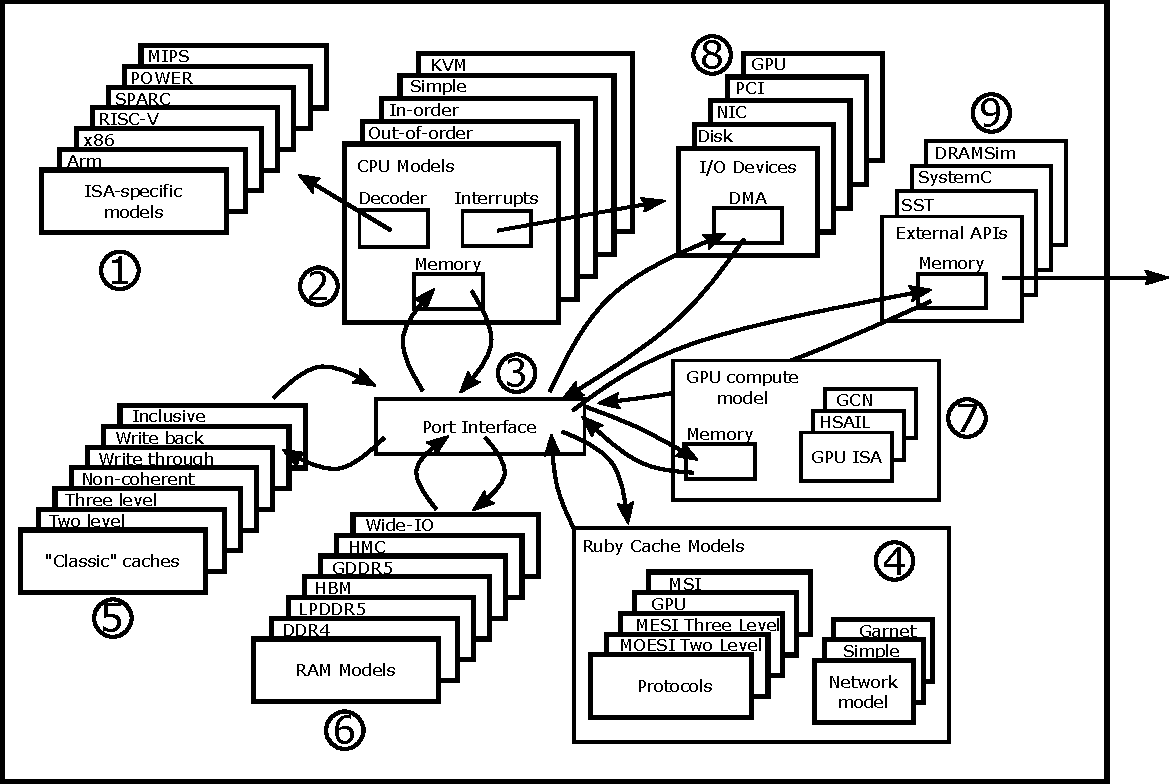
\includegraphics[width=\textwidth]{fig/gem5-big-picture}
  \caption{An overview of gem5's architecture. Its modular components allow any of each model type to be used in system configuration via Python scripts. Users can choose the fidelity of the memory system, CPU model, etc. while being able to select any ISA, devices, etc. The port interface allows any memory component to be connected to any other memory component as specified by the Python script. Details of each of these simulator components are discussed in Section~\ref{sec:main-features}}
  \label{fig:gem5-big-picture}
\end{figure*}

The gem5 simulator has modular support for multiple ISAs (see Figure~\ref{fig:gem5-big-picture}~\textcircled{1}).
gem5 currently supports Arm, GPU ISAs, MIPS, Power, RISC-V, SPARC, and x86.
These ISAs not only include the details to execute each instruction, but also the system-specific devices necessary for full system simulation.
There is robust full system support for Linux on Arm and x86 and many other ISAs have some level of full system support.

All of these ISAs can be used with any of gem5's CPU models as the CPU models are designed to be ISA-agnostic (Figure~\ref{fig:gem5-big-picture}~\textcircled{2}).
gem5 includes four different CPU models which span the fidelity performance continuum.
The highest performance CPU model is based on the kernel virtual machine (KVM) and leverages hardware virtualization to execute \emph{at native speeds}~\cite{full-speed-ahead}.
Although the KVM CPU model can execute at native speed, it does not model the timing of execution or memory.
gem5 also contains ``simple'' CPU models which are single-cycle models that can be used for memory system studies or other studies that do not require high-fidelity execution models.
Finally, gem5 contains a detailed in-order CPU model (the ``minor'' CPU) and an out-of-order CPU model (the ``O3'' CPU).

Underlying the memory system model in gem5 is a modular port interface which allows any component that implements the port API to be connected to any other component implementing that API ( Figure~\ref{fig:gem5-big-picture}~\textcircled{3}).
This allows models designed for one system to be easily used in other system designs.

There are two different cache systems in gem5: Ruby (Figure~\ref{fig:gem5-big-picture} \textcircled{4}), which models cache coherence protocols with high fidelity, and the ``classic'' caches (Figure~\ref{fig:gem5-big-picture}~\textcircled{5}).
Ruby enables user-defined cache coherence protocols, though gem5 includes many protocols out of the box.
%There are now 12 unique protocols including GPU-specific protocols~\cite{viper}, research protocols like token coherence~\cite{token-coherence} and region-coherence protocols~\cite{Power2012hsc}, and teaching protocols~\cite{coherence-primer}.
Users can also choose to use the detailed Garnet network mode~\cite{garnet-2} when using Ruby caches which offers cycle-level detail for the on-chip network.

The classic caches have a single hard-coded hierarchical MOESI coherence protocol.
However, this cache model is easily composable allowing users to construct hierarchical cache topologies without worrying about the correctness of the coherence protocol.
Both Ruby and the classic caches can be used with any CPU model, any ISA, and any memory controller model.

The gem5 simulator also includes an event-driven DRAM model (Figure~\ref{fig:gem5-big-picture}~\textcircled{6}).
This DRAM model is easily configurable with the timing parameters for a variety of different DRAM controllers including DDR3, DDR4, GDDR, HBM, HMC, LPDDR4, LPDDR5, and others.
Although this is not a cycle-accurate DRAM model like DRAMSim~\cite{} or Ramulator~\cite{}, it is nearly as accurate while providing more flexibility and higher performance~\cite{hansson-ispass-paper}

In addition to CPU models, gem5 also includes a cycle-level compute-based GPU~\cite{} (Figure~\ref{fig:gem5-big-picture}~\textcircled{7}).
This GPU model does not support graphics applications, but supports many compute applications based on the heterogeneous system architecture (HSA) and ROCm runtime.
The GPU model is based on AMD's Graphics Core Next architecture.
The GPU model has a modular ISA similar to the CPU model in gem5, and can be extended to support other GPU ISAs in the future.

An important component to full system simulation is supporting I/O and other devices (Figure~\ref{fig:gem5-big-picture}~\textcircled{8}).
gem5 supports many system-agnostic devices such as disk controllers, PCI components, ethernet controllers, etc. and system-specific devices such as the Arm GIC and SMMU and x86 PC devices.
Additionally, gem5 contains support for a ``fake'' graphics GPU to enable simulating applications that depend on graphics APIs.

Finally, gem5 has been integrated with other computer architecture simulator systems to enable users with models in other simulator systems to use gem5's features (Figure~\ref{fig:gem5-big-picture}~\textcircled{9}).
For instance, gem5 has been integrated with the System Simulation Toolkit (SST)~\cite{} which uses gem5's detailed CPU models in conjunction with SST's multi-node modeling capabilities.
The IEEE standard SystemC API~\cite{} has also been integrated with gem5 to enable users with SystemC models to use them as gem5 components.

Although there are many computer architecture simulators, and many of these are open source with features that overlap with gem5, gem5 is a unique simulation infrastructure.
\begin{itemize}
    \item gem5 is \emph{dynamically configurable} through a robust Python-based scripting interface. Most other simulators are configured statically with flat text files (e.g., json) or at compilation time. On the other hand, gem5 allows users to simulate complex systems much more easily by using object-oriented Python scripts to compose simpler systems into more complex ones.
    \item gem5 is \emph{extensible} through a clean model API. gem5 has over 300 models and adding new models is straightforward and well documented.
    \item gem5 is a \emph{full system} simulator. Its high-fidelity models can support booting unmodified operating systems and running modified applications with cycle-level statistics.
    \item gem5 is a \emph{community-driven} and \emph{frequently updated} project. The gem5 community is thriving. Since its original release nine years ago, there have been over 250 unique contributors and over 7500 commits. Even in the last six months, gem5 has had over 850 commits and 50 unique contributors.
\end{itemize}

\subsection{Becoming part of the gem5 community}

As a reader of this paper, you are already becoming part of the gem5 community!
Anyone who uses gem5 or contributes in any way is part of the gem5 community.
Contributing can be as simple as sending a question on the gem5 mailing list\footnote{\url{http://www.gem5.org/mailing_lists/}} or as complex as adding a new model to the upstream codebase.
Below, we discuss some of the common ways to use gem5 and become part of the community.

\subsubsection{For researchers}

Currently, the most common use case for gem5 is in computer architecture research.
In this case, researchers download the gem5 source, build the simulator, and then add their own device models on top of the models included in upstream gem5.
This use case requires deep knowledge of the core simulation frameworks of gem5.
However, we are working to make it easier to get started developing and researching with gem5 through efforts like the Learning gem5 materials and online course~\ref{sec:learning}.

After using gem5 in their research, we encourage these users to contribute their improvements and fixes to the gem5 back to the mainline codebase.
Not only does this improve gem5 for others, but it also makes reproducing research results easier.
Rather than managing many local changes and trying to keep up with new releases of gem5, when code is contributed upstream it is the responsibility of \emph{others in the community} to ensure that the code stays up to date.
Additionally the gem5 project employs a permissive BSD license to lower the barrier of contribution for both academics and industry researchers.

\subsubsection{For students and teachers}

The gem5 simulator can be used as a tool for teaching computer architecture as well.
Historically, there has been a very steep learning curve for using gem5 even for simple experiments.
However, with the improved documentation, this learning curve is coming down.

We will be continuing to improve gem5 with the goal of making it easier for both students and teachers to use to learn and teach computer architectures concepts.
For example, the new Learning gem5 material created for the online course will include a set of example exercises that we hope can be used in both undergraduate and graduate computer architecture courses.
Additionally, we are working to develop a new GUI-based frontend for gem5 and to develop known-good models that do not required deep knowledge of simulator internals to configure and use.
